\documentclass{article}
\usepackage[T1]{fontenc}
\usepackage{lmodern}
\usepackage{graphicx}
\usepackage{amsmath,amssymb}
\usepackage[a4paper,margin=2cm]{geometry}
\usepackage[absolute,overlay]{textpos}
\setlength{\TPHorizModule}{1mm}
\setlength{\TPVertModule}{1mm}
\usepackage[indonesian]{babel}
\usepackage{hyperref}
\setlength{\emergencystretch}{2em}
% unit: Halaman 55

\begin{document}

% === Halaman 55 (python/native) ===

Contoh substitusi di dalam block cipher AES:

55

Input: 23  (Hexadecimal)

Output: 26  (Hexadecimal)

Cara substitusi;

-

Cari perpotongan baris 2

     dengan kolom 3

-    hasilnya adalah 26

% deskripsi: gambar native xref 222
\noindent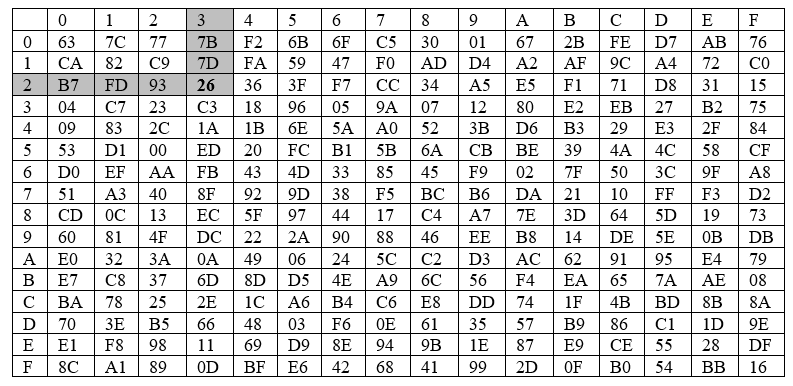
\includegraphics[width=0.85\textwidth]{../../images/python/page_055_img_01.png}

\end{document}
